
%%%%%%%%%%%%%%%%%%%%%%%%%%%%%%%%%%%%%%%%%%%%%%%%%%%%%%%%%%%
%% Capítulo 2: Polinomios Ortoganles Clásicos            %%
%%%%%%%%%%%%%%%%%%%%%%%%%%%%%%%%%%%%%%%%%%%%%%%%%%%%%%%%%%%


En el capítulo \ref{chap:introduccionPO} hemos mostrado una amplia introducción a la ortogonalidad y presentado ejemplos concretos de polinomios ortogonales. En este capítulo presentaremos las familias concretas de polinomios ortogonales más importantes: los \textit{polinomios ortogonales clásicos}. Estos son los polinomios de Hermite, Laguerre, Jacobi y Bessel. Estas familias presentan la peculiaridad de ser las únicas que verifican ciertas propiedades, entre las que destaca la \textit{ecuación diferencial de Pearson}. Estos polinomios, entre otras disciplinas pueden ser encontrados en problemas de Sturm-Liouville cuando se utilizan ecuaciones diferenciales hipergeométricas.

\begin{figure}[h]
    \centering
    \begin{tabular}{ccc}
        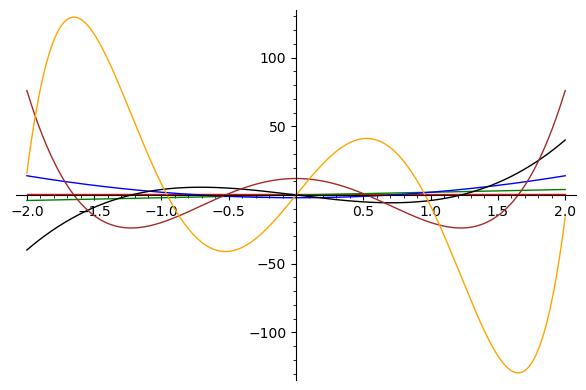
\includegraphics[width=5cm]{img/C2/hermite.png} & 
        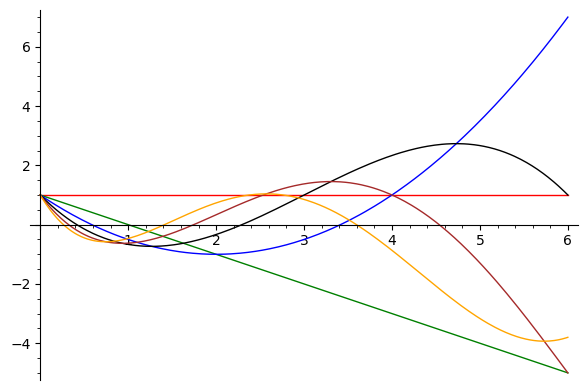
\includegraphics[width=5cm]{img/C2/laguerre.png} &
        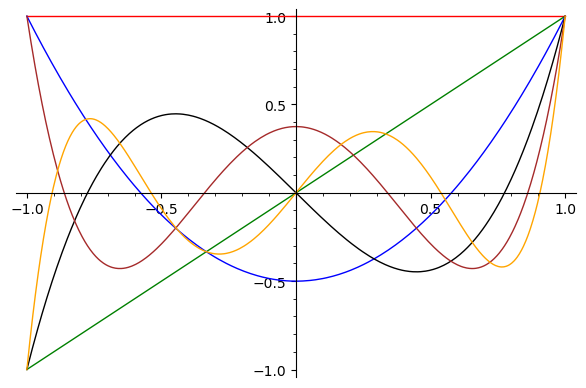
\includegraphics[width=5cm]{img/C2/jacobi.png} \\
        (a) Hermite $H_n$ & (b) Laguerre $L^{(0)}_n$ & (c) Jacobi $J^{(0,0)}_n$ 
    \end{tabular}
    \caption{Polinomios Ortogonales Clásicos}
    \label{img:graficas-clasicos}
\end{figure}

En las imágenes \ref{img:graficas-clasicos} podemos ver la representación gráfica, para parámetros concretos que definiremos próximamente, de los polinomios ortogonales de Hermite, Laguerre y Jacobi. Estas tres son las familias que mayor atención recibirán de nuestra parte al ser aquellas cuya ortogonalidad se manifiesta en intervalos reales.